\section{01 - Intro}

\begin{definition}{Business IT-Risks}
    \begin{itemize}
        \item Ransom Demand
        \item Fraud
        \item Espionage
        \item Violation of Regulations
        \item Misuse of Computing Resources
        \item Reputation Loss
        \item System Outage
        \item Sabotage
        \item Data Loss
        \item Brand Misuse
    \end{itemize}
\end{definition}

\begin{concept}{Problems - Overview} and their impact on data availability
\paragraph{Physisch}
\textbf{unabsichtlich}
\begin{itemize}
    \item Naturkatastrophen
    \item Feuer
    \item Ausfall
    \item Kaffee auf Server
\end{itemize}

\textbf{absichtlich/bösartig}
\begin{itemize}
    \item Feuer
    \item Vandalismus
    \item Garantie läuft aus -> absichtlich langsamer
    \item Social Engineering
\end{itemize}

\paragraph{Virtuell}
\textbf{unabsichtlich}
\begin{itemize}
    \item Bitflip
    \item Config Fehler
    \item Bugs im SW
    \item Phishing klicken
\end{itemize}

\textbf{absichtlich/bösartig}
\begin{itemize}
    \item DDoS
    \item Malware
    \item Ransomware
    \item Phishing senden
    \item Trojaner
\end{itemize}
\end{concept}

\begin{theorem}{Countermeasures - Overview}

\textbf{Disaster Recovery}
    \begin{itemize}
        \item Offline backup solutions
        \item Restoring from images
    \end{itemize}

\textbf{Access Control}
    \begin{itemize}
        \item Restricted Access Rights
        \item Multi-Factor Authentication
        \item Firewalls
        \item Traffic Management Solutions
    \end{itemize}

\textbf{Physical Protection}
    \begin{itemize}
        \item Physical Access Control (locks, fences, etc.)
        \item Fire Protection (extinguishers, alarms, etc.)
        \item Monitoring (CCTV, Guards etc.)
    \end{itemize}

\textbf{Training Processes}
    \begin{itemize}
        \item Employee Training
        \item Four eyes principle
        \item Automation of routine processes
        \item Monitoring
        \item Preventive maintenance
    \end{itemize}

\textbf{Redundancy}
    \begin{itemize}
        \item Uninterruptable Power Supplies
        \item High Availability setups
        \item Load Balancing
        \item Redundant data center
        \item Redundant network connections
    \end{itemize}
\end{theorem}

\begin{formula}{Recovery Plan and Test}

    
\includegraphics[width=\linewidth]{recovery_plan_test.png}

    \textbf{Recovery Plan} - description of what to do if something goes wrong
    \begin{itemize}
        \item Roles and responsibilities
        \item Processes
        \item Contact details
        \item Technical instructions
    \end{itemize}

    \textbf{Recovery Test} - testing the recovery plan
    \begin{itemize}
        \item Theoretical dry run
        \item Practical tests
        \begin{itemize}
            \item turn off a server or DC
            \item restore data from backup
        \end{itemize}
    \end{itemize}
\end{formula}

\begin{concept}{Goals of IT Security}

Most measures in Information Security have one of the three following high-level goals:
\begin{itemize}
    \item Ensure data is confidential
    \item Ensure data is not corrupted
    \item Ensure data and systems are available
\end{itemize}

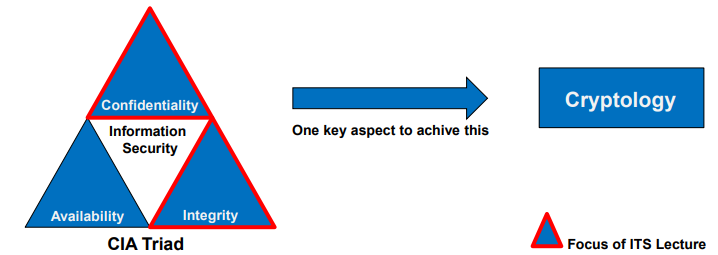
\includegraphics[width=\linewidth]{goals_of_IT_security.png}
\end{concept}

\raggedcolumns


\section{Overview of IT Security}

\subsection{Introduction to IT Security}

\begin{definition}{Key IT Security Goals}\\
Information security is based on three fundamental principles, commonly known as the CIA triad:
\begin{itemize}
    \item \textbf{Confidentiality} - Ensuring data is only accessible to authorized users
    \item \textbf{Integrity} - Ensuring data is not modified in an unauthorized way
    \item \textbf{Availability} - Ensuring systems and data are accessible when needed
\end{itemize}
\end{definition}

\begin{concept}{Business IT Risks}\\
Organizations face numerous security threats that can impact business operations:
\begin{itemize}
    \item Data loss
    \item System outage
    \item Espionage
    \item Sabotage
    \item Reputation loss
    \item Misuse of computing resources
    \item Violation of regulations
    \item Fraud
    \item Brand misuse
    \item Ransom demands
\end{itemize}
These risks can have significant financial, operational, and reputational impacts.
\end{concept}

\subsection{Security Frameworks and Controls}

\begin{concept}{Security Control Frameworks}\\
Security frameworks provide structured approaches to implementing security controls:
\begin{itemize}
    \item \textbf{CIS Controls} - Prioritized set of actions to protect organizations
    \item Controls are typically organized in implementation groups based on difficulty and impact
    \item Focus on preventing the most common attack vectors first
\end{itemize}
\end{concept}

\begin{definition}{Types of Security Measures}\\
Security measures can be categorized based on their focus:
\begin{itemize}
    \item \textbf{Preventive} - Block threats before they occur (firewalls, access controls)
    \item \textbf{Detective} - Identify when a breach has occurred (IDS, audit logs)
    \item \textbf{Corrective} - Mitigate damage after an incident (backups, incident response)
\end{itemize}
\end{definition}

\subsection{Disaster Recovery}

\begin{concept}{Business Continuity Management}\\
Disaster recovery and business continuity planning are essential for maintaining availability:
\begin{itemize}
    \item \textbf{Recovery Plan} - Detailed procedures for recovering from incidents
    \item \textbf{Recovery Tests} - Regular testing of recovery procedures
    \item \textbf{Redundancy} - Duplicate systems, power supplies, and network connections
    \item \textbf{Offline backups} - Protection against ransomware and other threats
\end{itemize}
\end{concept}

\begin{KR}{Disaster Recovery Planning}\\
\paragraph{Initial Assessment}
\begin{itemize}
    \item Identify critical systems and data
    \item Determine acceptable recovery time objectives (RTO)
    \item Determine acceptable recovery point objectives (RPO)
\end{itemize}

\paragraph{Plan Development}
\begin{itemize}
    \item Document recovery procedures
    \item Assign roles and responsibilities
    \item Include contact details for all relevant parties
    \item Develop technical instructions for restoration
\end{itemize}

\paragraph{Testing}
\begin{itemize}
    \item Conduct regular theoretical dry runs
    \item Perform practical tests (e.g., server shutdown, data restoration)
    \item Update procedures based on test results
\end{itemize}

\paragraph{Regular Review}
\begin{itemize}
    \item Review and update plans regularly
    \item Consider changes in infrastructure, personnel, and threats
\end{itemize}
\end{KR}

\begin{example}
A medium-sized company implements a disaster recovery plan for their customer database. They define an RTO of 4 hours and an RPO of 15 minutes, meaning they need to restore service within 4 hours with no more than 15 minutes of data loss. To achieve this, they implement a combination of hourly differential backups with continuous transaction log shipping to a standby site. Regular recovery tests are scheduled quarterly to ensure the plan remains effective.
\end{example}

\section{Introduction to Security and Cryptology}

\subsection{Ziele der Kryptographie}

\begin{definition}{Ziele der Kryptographie}\\
    Die Kryptographie verfolgt vier Hauptziele:
    \begin{itemize}
        \item \textbf{Confidentiality} Only readable by desired receiver.
        \item \textbf{Integrity} The receiver can determine if the message has been altered.
        \item \textbf{Authenticity} The receiver can validate its origin.
        \item \textbf{Freshness} The message is new and cannot be resent.
    \end{itemize}
\end{definition}

\subsection{Encryption and Properties}

\begin{concept}{Encryption}\\
    Encryption is a transformation from P (plaintexts) to C (ciphertexts) under control of some key, chosen from K (key space).
    
    The idea is to have a whole family of transformations, where each key gives a different transformation.
    \begin{itemize}
        \item $c = E(k, p) = E_k(p)$
        \item $p = D(k, c) = D_k(c)$
    \end{itemize}
    
    Each transformation must be reversible. It follows that $|C|$ can not be smaller than $|P|$. In fact most often we have $P = C$.
\end{concept}

% TODO: Add encryption/decryption diagram with key, plaintext, cipher components

\subsection{Passive Attacks (Eve) - Type of Attacks}

\begin{definition}{Attack Types}\\
    \begin{itemize}
        \item \textbf{Cypher-Text-Only Attack} Bad Encryption $\rightarrow$ Find out plaintext or even the key
        
        Maybe the encryption isn't good and Eve can find out the plaintext just by looking at ciphertexts.
        
        \item \textbf{Chosen-Plain-Text attack} Encrypt machine stolen $\rightarrow$ Find out plaintexts
        
        Maybe someone stole Alice's encryption machine for a few hours. Then Eve can encrypt some plaintexts of her choice and maybe find the plaintexts to ciphertexts she has intercepted.
        
        \item \textbf{Chosen-Ciphertext attack 1} Decrypt machine stolen $\rightarrow$ Learn about the key
        
        Someone has stolen Alice's decryption machine for a few hours. How much can Eve learn about the key by being allowed to feed ciphertexts to the machine?
        
        \item \textbf{Chosen-Ciphertext attack 2} Decrypt machine stolen $\rightarrow$ Learn about the key
        
        Someone has stolen Alice's decryption machine. How much can Eve learn about the key by being allowed limited information about decryption.
    \end{itemize}
\end{definition}

\subsection{Cryptographic Work Factor}

\begin{definition}{Work Factor}\\
    The number of times it takes to come upon the correct key is called (cryptographic) work factor.
    \begin{itemize}
        \item Work factor (WF) = average number of keys to try
        \item Work factor is usually given in bits: $\log_2(n)$, $n = key\ space\ size$
    \end{itemize}
\end{definition}

\begin{formula}{Entropy}\\
    Entropy is maximal if all outcomes are equally likely
    $$H = \sum_{i=1}^{n} p(i) \cdot \log_2 \left(\frac{1}{p(i)}\right)$$
    
    $$H_{binary} = \sum_{i=1}^{n} \frac{1}{n} \log_2(n) = \log_2(n)$$
\end{formula}

\begin{concept}{Entropy of Cryptographic Keys}\\
    Cryptographic keys are typically created with random generators, so they can be considered as elements of a random variable.
    
    What's the entropy of a key with 128-bit?
    \begin{itemize}
        \item Independent with equal probability: $128 \cdot 1 = 128$ bits
        \item Dependent with inequal probability: $p(0) = 0.25, p(1) = 0.75 \rightarrow 128 \cdot 0.81 \approx 104$ bits
    \end{itemize}
\end{concept}

\begin{theorem}{Relation between entropy and work factor}\\
    \begin{itemize}
        \item Work Factor $\approx$ entropy, key size = max. entropy $\approx$ max. work factor
    \end{itemize}
\end{theorem}

\subsection{Security Models}

\begin{definition}{Information-theoretically secure}\\
    Intercepting a ciphertext tells you nothing about the plain
\end{definition}

\begin{definition}{Computationally secure}\\
    Work factor $\approx$ key entropy
\end{definition}

\subsection{Vernam Cipher (a.k.a. One-Time-Pad)}

\begin{concept}{One-Time-Pad}\\
    \begin{itemize}
        \item Key $K$: Independent bits with equal probability
        \item $C_X = K_X \oplus P_X$
        \item Each key may be used once
        \item Same Key used multiple times: $P_1 \oplus P_2 = C_1 \oplus C_2$
    \end{itemize}
\end{concept}

% TODO: Add One-Time-Pad diagram showing XOR operations

\subsection{Random Oracle Model}

\begin{concept}{Random Oracle Model}\\
    \begin{itemize}
        \item Different inputs give random unrelated outputs
        \item If $A$ leads to $B$ then $A$ always leads to $B$
    \end{itemize}
\end{concept}

\subsection{Modern Ciphers with One key}

\begin{concept}{Modern Ciphers}\\
    \begin{itemize}
        \item Same key is used to encrypt and decrypt
        \item Wrong key gives high-entropy output: can tell when correct key used
        \item Good modern ciphers: key entropy $\approx$ work factor
        \item Cryptographic workhorse today: AES
    \end{itemize}
\end{concept}

\subsection{Properties of Modern Ciphers}

\begin{remark}
    \begin{itemize}
        \item Information-theoretical security is out of question
        \item Next best thing: computational security
        \item No cipher is known that can be proved to be computationally secure
        \item Cipher created $\rightarrow$ public review $\rightarrow$ gains acceptance
    \end{itemize}
\end{remark}